\section{Tutorials}
Here I'll provide a few tutorials on how to use SolidWorks to create the assemblies needed for 
the parametric studies.

\begin{itemize}
    \item \href{https://youtu.be/PvouSPWoutg?si=g4lY9noGS2_bfpGE}{SolidWorks basics of flow simulation}
    \item All you need guide for parametric studies in solidwoks for ACS.
\end{itemize}

\section{SolidWorks basics}
It all comes down to having simple models, that are full and having whole body in one part and 
canards in another. This is needed for the parametric studies assembly. \\\\
We conducted a few simulations for Sternik 1.5 model, which were dependant on 4 parameters:
\begin{itemize}
    \item Canard 1 angle
    \item Canard 2 angle
    \item Angle of attack
    \item Angle of sideslip
\end{itemize}
In whole phase of early studies, we would only paremetrise 1 or 2 parameters, since 
it allowed us to generate graphs which we could understand and analyze. \\\\
Together with Piotrek, we used Origin Pro for data analysis, which allowed us to generate cool 3d
heatmaps, which were very useful for understanding the forces and moments acting on the model. \\\\
Bellow you will find a few screenshots of the simulations we conducted and the heatmaps we generated.
Then I will write about problems we encountered and how we solved them.\\\\
IMPORTANT!!! Positive values of canard angles mean that cannard is rotated in couter clockwise 
direction. This means that if both canards have same value of angle, then high value of 
torque in Y(roll) should be observed and for torque X, Z should be near 0. \\\\

\section{First simulation - Sternik 1.5}
This one is just the images of pressures etc for a very particular mesh. Just to document how it 
looks.

\begin{figure}[H]
    \centering
    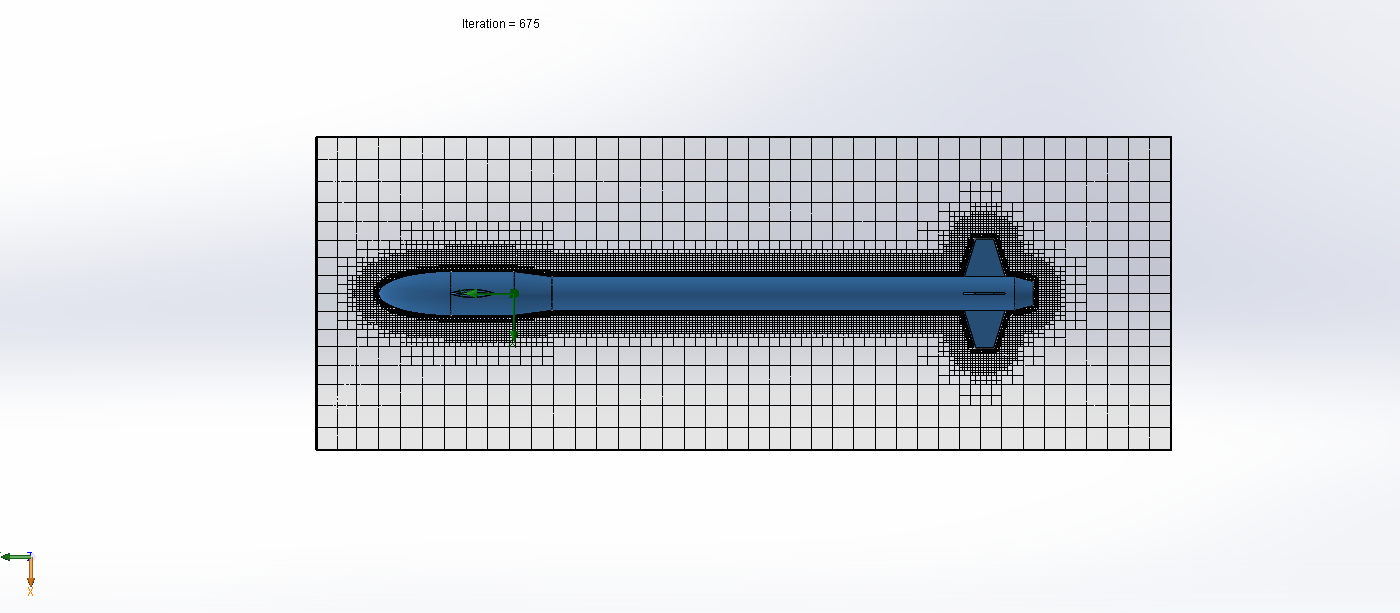
\includegraphics[width=\textwidth]{FirstImages00Sternik15/HelloWorldSimulation2Mesh.png}
    \caption{Sternik 1.5 model}
\end{figure}


\begin{figure}[H]
    \centering
    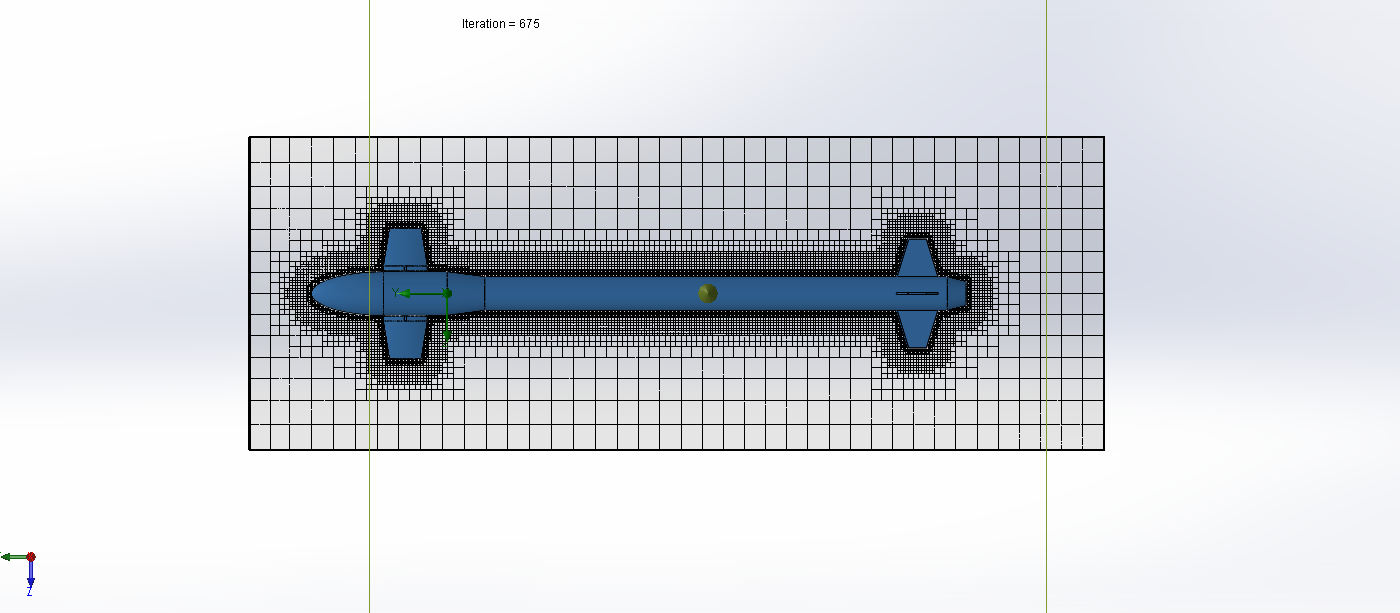
\includegraphics[width=\textwidth]{FirstImages00Sternik15/HelloWorldSimulation2MeshL.png}
    \caption{Sternik 1.5 model}
\end{figure}

\begin{figure}[H]
    \centering
    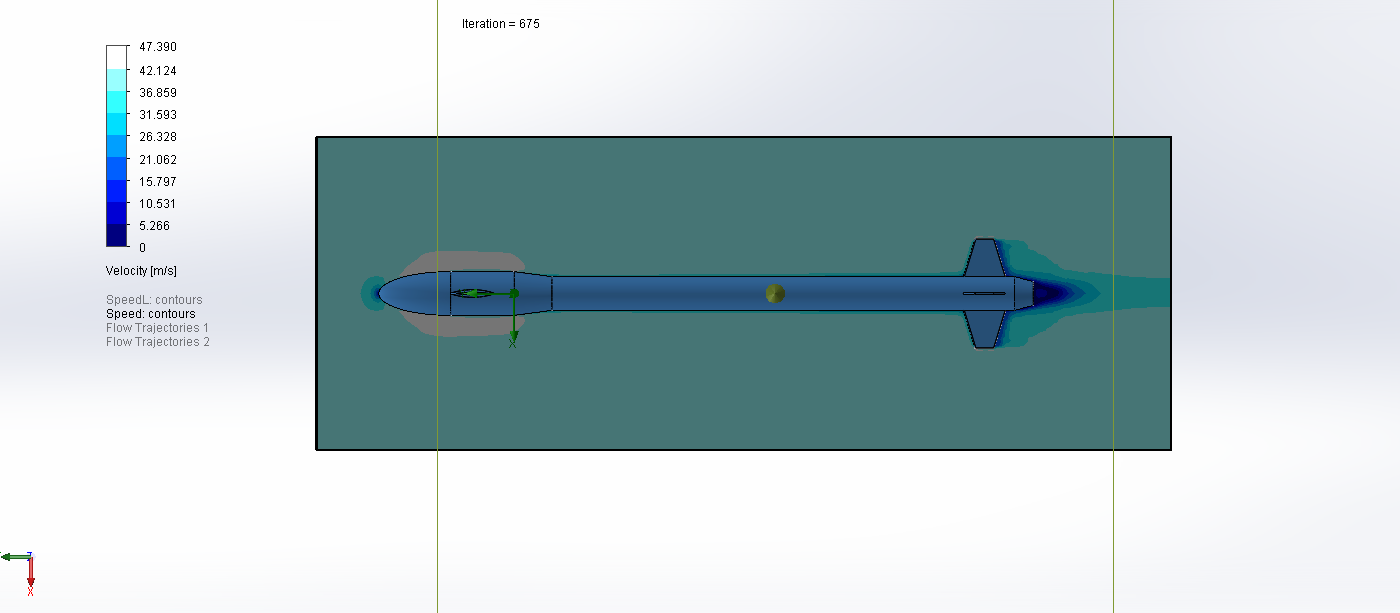
\includegraphics[width=\textwidth]{FirstImages00Sternik15/HelloWorldSimulation2Speed.png}
    \caption{Sternik 1.5 model}
\end{figure}


\begin{figure}[H]
    \centering
    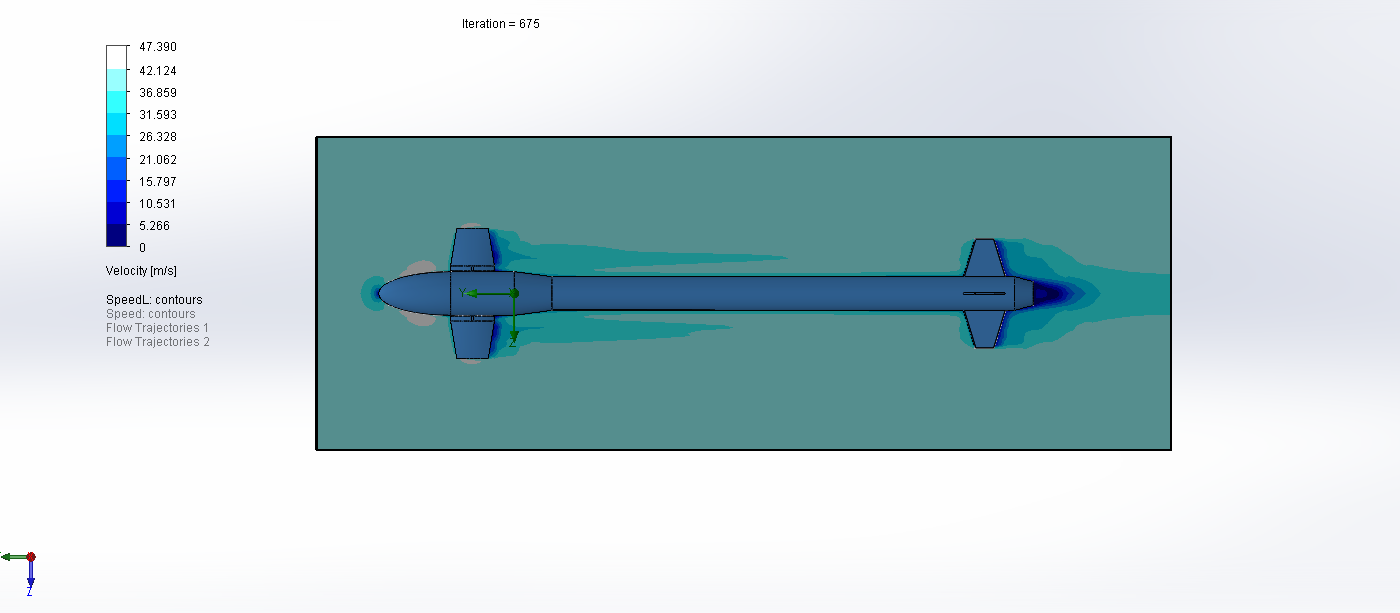
\includegraphics[width=\textwidth]{FirstImages00Sternik15/HelloWorldSimulation2SpeedL.png}
    \caption{Sternik 1.5 model}
\end{figure}


\begin{figure}[H]
    \centering
    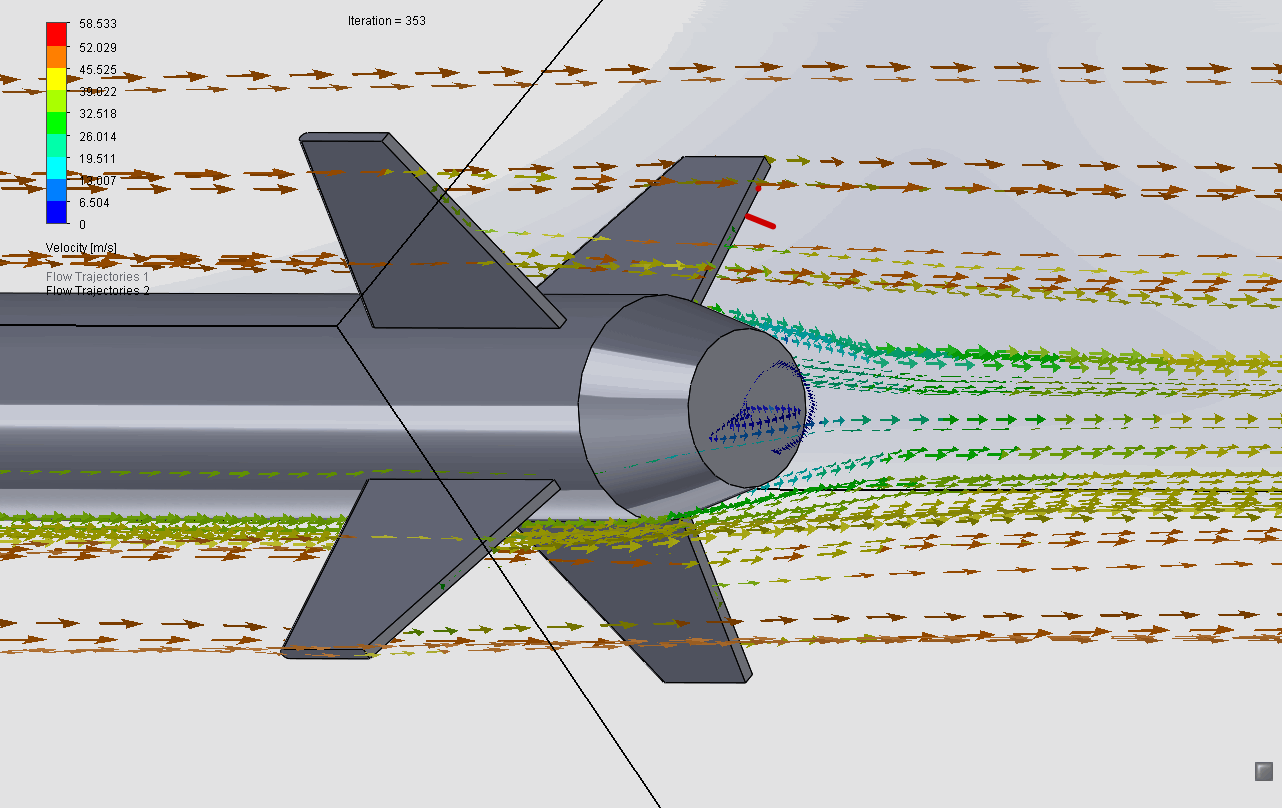
\includegraphics[width=0.8\textwidth]{FirstImages00Sternik15/Animation2.png}
    \caption{Sternik 1.5 model}
\end{figure}

\begin{figure}[H]
    \centering
    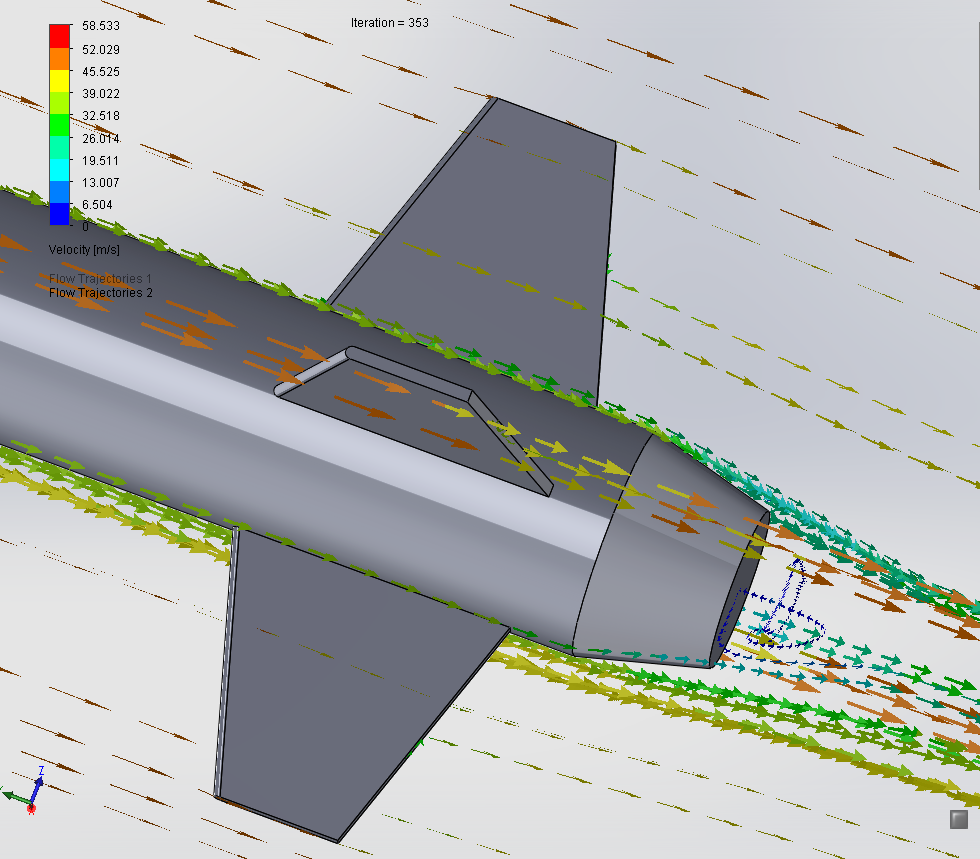
\includegraphics[width=0.8\textwidth]{FirstImages00Sternik15/strzalki1.png}
    \caption{Sternik 1.5 model}
\end{figure}

\section{First parametric for all values done by Piotrek - Sternik 1.5}
This one genereted all forces and moments for (-30, 30) degrees for both canards. You can find 
results in the Parametric\_Study\_obie\_lotki\_Piotrek\_PIERWSZA.xlsx\ file. \\\\
We didnt do any heatmaps for this one, since we were just testing the parametric study feature.

\section{Second parametric by Manfred and Piotrek - Sternik 1.5}
This one was done for (0, 30) degrees for both canards. You can find results in the 
CFDPiotrekManfredACS.xlsx file. \\\\
This time heatmaps were generated, which allowed us to understand the forces and moments acting on
the model. We then analised the results and with Jacek and Piotrek came to a conclusion that
it all looks good.

\begin{figure}[H]
    \centering
    \includegraphics[width=\textwidth]{PiotrekManfred0-30/torqueX.png}
    \caption{Sternik 1.5 model}
\end{figure}

\begin{figure}[H]
    \centering
    \includegraphics[width=0.8\textwidth]{PiotrekManfred0-30/torqueY.png}
    \caption{Sternik 1.5 model}
\end{figure}

\begin{figure}[H]
    \centering
    \includegraphics[width=0.8\textwidth]{PiotrekManfred0-30/torqueZ.png}
    \caption{Sternik 1.5 model}
\end{figure}

\begin{figure}[H]
    \centering
    \includegraphics[width=0.8\textwidth]{PiotrekManfred0-30/forceY.png}
    \caption{Sternik 1.5 model}
\end{figure}
The important take away from this is that we were able to generate heatmaps for all forces that
made sense. \\\\
Also we can see the local maximums and mininums for torques for the angle of 20 degrees. Jacek said
that this is a good sign, since in literature there is said that maximum should be at around that
value.
\newpage
\section{Same parametic study for Sternik 1.5 but with different mesh by Manfred}
This one is basicly the same as the previous one, but with a different mesh. I wanted to replicate
the results from the previous study and learn how to make parametric studies by myself. The results
are ParametricStudy80k0-30-30-30\_Manfred.xlsx. \\\\
The heatmaps are not as good as the previous ones, but they still show the same trends. 
Maxiumums and minimums are not visible this time, but this could be because of baddly made mesh.
The quality of mesh was better tho, it was 80k cells and 16k cells for the boundary layer.\\\\
IMPORTANT TAKE AWAY. In solidworks you cannot change the parameter angle in assembly in sketch to 
negative value. Thats why later we went for defeault being 90 degrees or by hand 10 and for 
-10 = 170 degrees. \\\\
Also comparison of the results from the previous study and this one is bellow.
\begin{figure}[H]
    \centering
    \includegraphics[width=0.8\textwidth]{Manfred0-30/torqueX.png}
    \caption{Sternik 1.5 model}
\end{figure}

\begin{figure}[H]
    \centering
    \includegraphics[width=0.8\textwidth]{Manfred0-30/torqueY.png}
    \caption{Sternik 1.5 model}
\end{figure}

\begin{figure}[H]
    \centering
    \includegraphics[width=0.8\textwidth]{Manfred0-30/torqueZ.png}
    \caption{Sternik 1.5 model}
\end{figure}

\begin{figure}[H]
    \centering
    \includegraphics[width=0.6\textwidth]{Manfred0-30/forceY.png}
    \caption{Sternik 1.5 model}
\end{figure}

\begin{figure}[H]
    \centering
    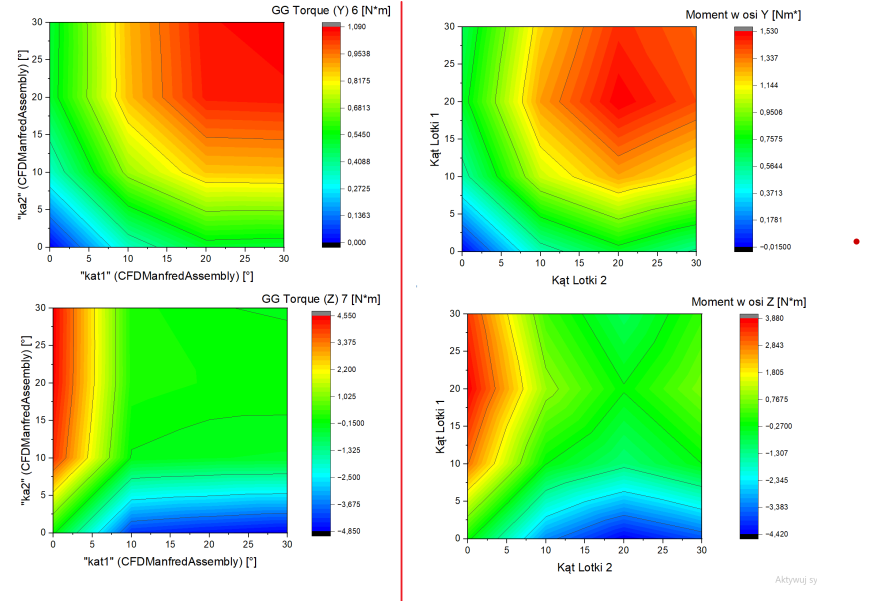
\includegraphics[width=0.8\textwidth]{Manfred0-30/vs.png}
    \caption{Sternik 1.5 model}
\end{figure}
Important take away is that the results are very similar, which is a good sign, but different 
meshes can give different results. \\\\
Also dont forget about negative values of angle not working.

\section{Similar study but for (-30; 30) (0; 30) angles for Sternik 1.5 by Manfred}
Basicly we wanted to make full bigger study, this time only 12k cells, so a small number, 
but resoults were similar and symetries would happen now. For symetric maps take into account
that the lower part of heatmap may have inverted colours. \\\\
The results are in the ParametricStudy12k\_-30-30\_0-30.xlsx file. \\\\

\begin{figure}[H]
    \centering
    \includegraphics[width=\textwidth]{Manfred-30-30/torqueX.png}
    \caption{Sternik 1.5 model}
\end{figure}

\begin{figure}[H]
    \centering
    \includegraphics[width=\textwidth]{Manfred-30-30/torqueY.png}
    \caption{Sternik 1.5 model}
\end{figure}

\begin{figure}[H]
    \centering
    \includegraphics[width=\textwidth]{Manfred-30-30/torqueZ.png}
    \caption{Sternik 1.5 model}
\end{figure}

\begin{figure}[H]
    \centering
    \includegraphics[width=\textwidth]{Manfred-30-30/forceX.png}
    \caption{Sternik 1.5 model}
\end{figure}

\begin{figure}[H]
    \centering
    \includegraphics[width=\textwidth]{Manfred-30-30/forceY.png}
    \caption{Sternik 1.5 model}
\end{figure}

\begin{figure}[H]
    \centering
    \includegraphics[width=\textwidth]{Manfred-30-30/forceZ.png}
    \caption{Sternik 1.5 model}
\end{figure}

\begin{figure}[H]
    \centering
    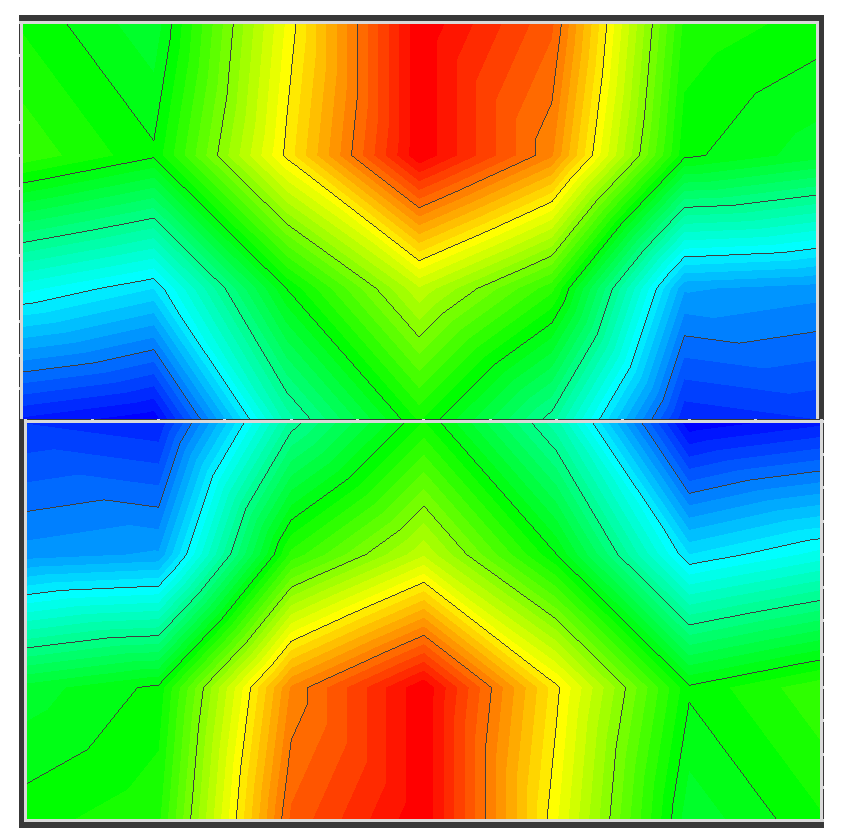
\includegraphics[width=\textwidth]{Manfred-30-30/invX.png}
    \caption{Sternik 1.5 model}
\end{figure}

\begin{figure}[H]
    \centering
    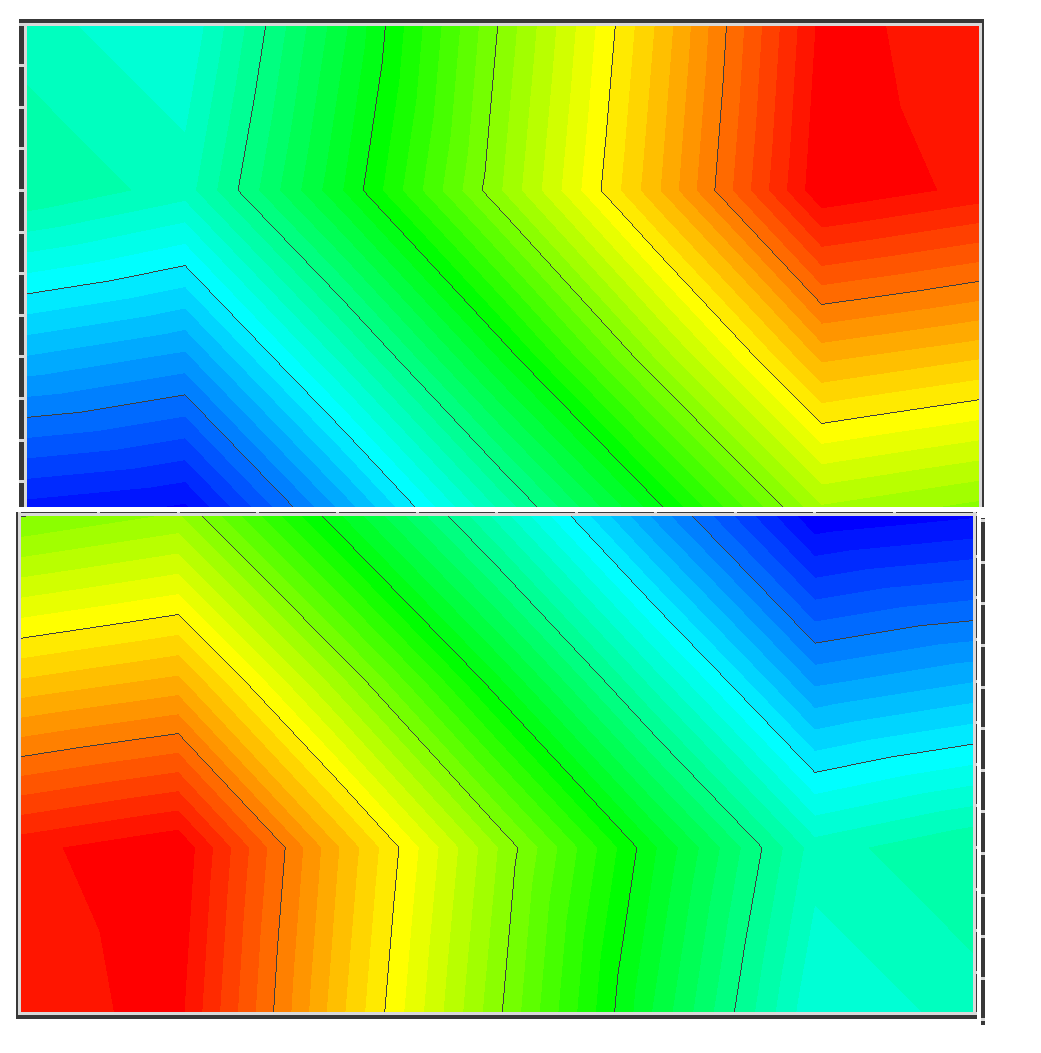
\includegraphics[width=\textwidth]{Manfred-30-30/invY.png}
    \caption{Sternik 1.5 model}
\end{figure}

\begin{figure}[H]
    \centering
    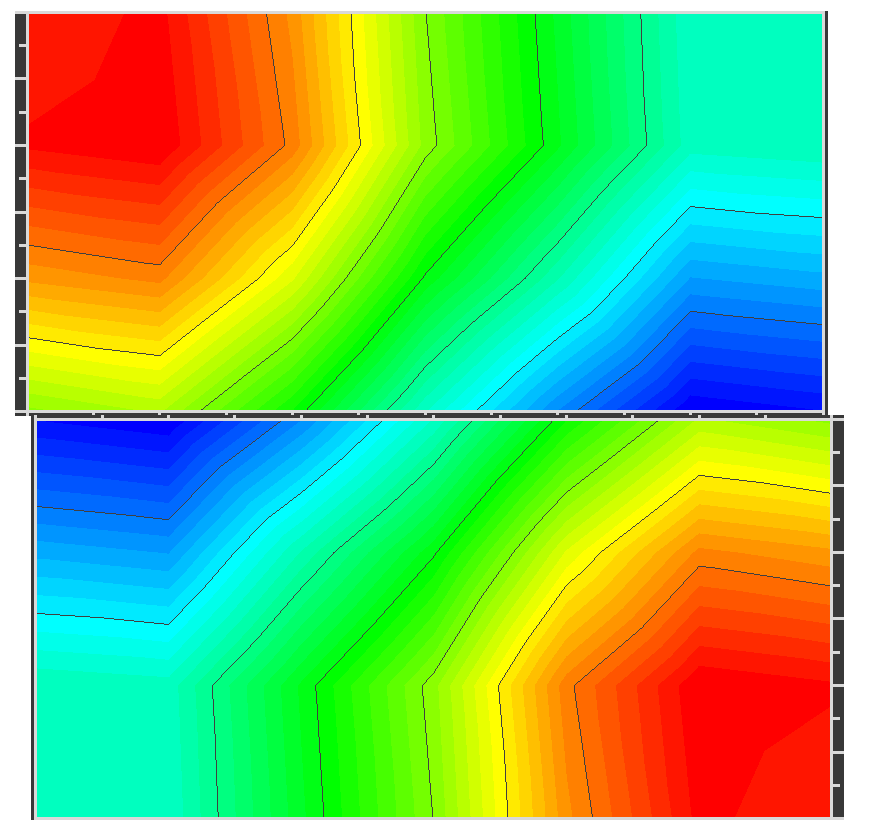
\includegraphics[width=\textwidth]{Manfred-30-30/invZ.png}
    \caption{Sternik 1.5 model}
\end{figure}
\newpage
\section{Parametric study for Sternik 1.5 for (-30; 30) (-30; 30) by Piotrek}
This time its a full study for all angles. I cant find the results but here are the heatmaps and 
mesh settings. \\\\

\begin{figure}[H]
    \centering
    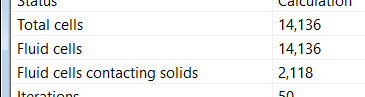
\includegraphics[width=0.8\textwidth]{Piotrek-30-30-30-30/cells.png}
    \caption{Sternik 1.5 model}
\end{figure}

\begin{figure}[H]
    \centering
    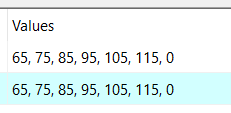
\includegraphics[width=0.8\textwidth]{Piotrek-30-30-30-30/range.png}
    \caption{Sternik 1.5 model}
\end{figure}

\begin{figure}[H]
    \centering
    \includegraphics[width=0.8\textwidth]{Piotrek-30-30-30-30/torqueX.png}
    \caption{Sternik 1.5 model}
\end{figure}

\begin{figure}[H]
    \centering
    \includegraphics[width=0.8\textwidth]{Piotrek-30-30-30-30/torqueY.png}
    \caption{Sternik 1.5 model}
\end{figure}

\begin{figure}[H]
    \centering
    \includegraphics[width=0.8\textwidth]{Piotrek-30-30-30-30/torqueZ.png}
    \caption{Sternik 1.5 model}
\end{figure}

\begin{figure}[H]
    \centering
    \includegraphics[width=0.8\textwidth]{Piotrek-30-30-30-30/forceX.png}
    \caption{Sternik 1.5 model}
\end{figure}

\begin{figure}[H]
    \centering
    \includegraphics[width=0.8\textwidth]{Piotrek-30-30-30-30/forceY.png}
    \caption{Sternik 1.5 model}
\end{figure}

\begin{figure}[H]
    \centering
    \includegraphics[width=0.8\textwidth]{Piotrek-30-30-30-30/forceZ.png}
    \caption{Sternik 1.5 model}
\end{figure}

For comparison, results of Torque X for same study but with angle of attack of 10 degrees are
bellow. As you can see, nothing of the old results is visible. We tried to analyze the results, but
only conclusion we came is that non linear nature of this problem is very hard to imagine. \\\\

\begin{figure}[H]
    \centering
    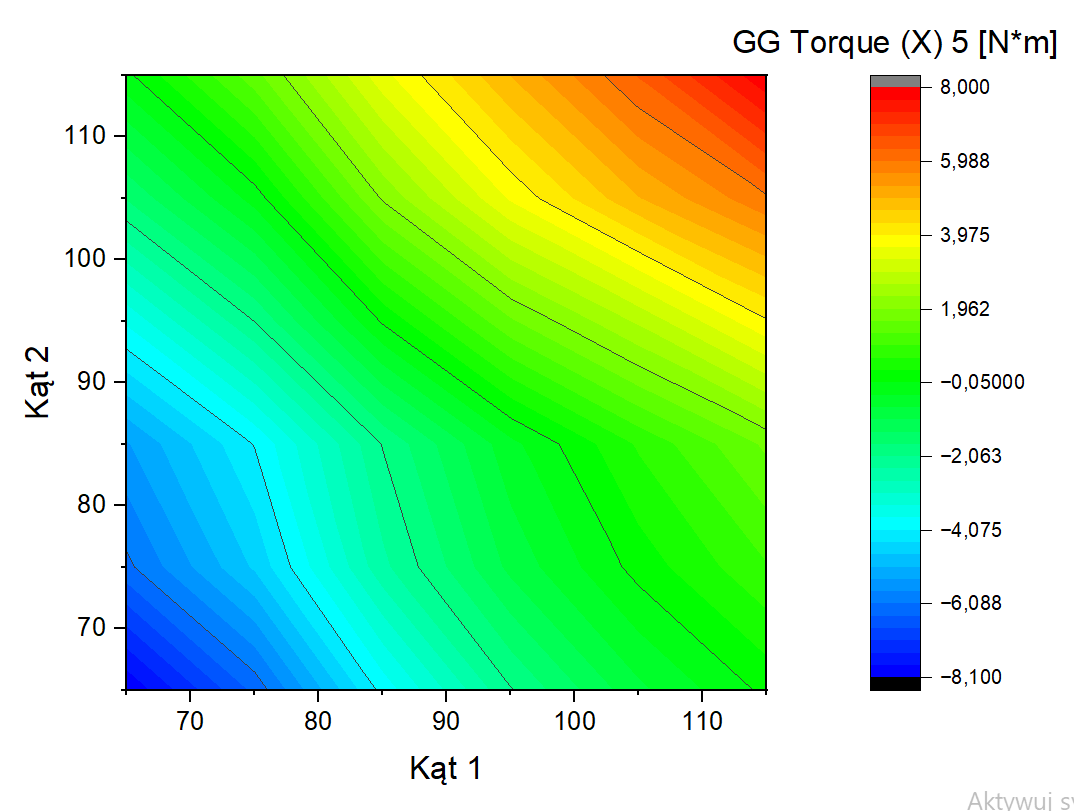
\includegraphics[width=0.8\textwidth]{Piotrek-30-30-30-30/plus10.png}
    \caption{Sternik 1.5 model}
\end{figure}


\newpage
\section{Parametric study for Sternik 1.5 with angle of attack and sideslip}
Here is where to change the parameters in general settings of the simulation. Just change it 
to 3D vector.\\\\
There are also how you should change the angles of attack and sideslip in parametric study. BUT 
WE WILL LATER DISCUSS WHY NOT TO DO THAT. \\\\

\begin{figure}[H]
    \centering
    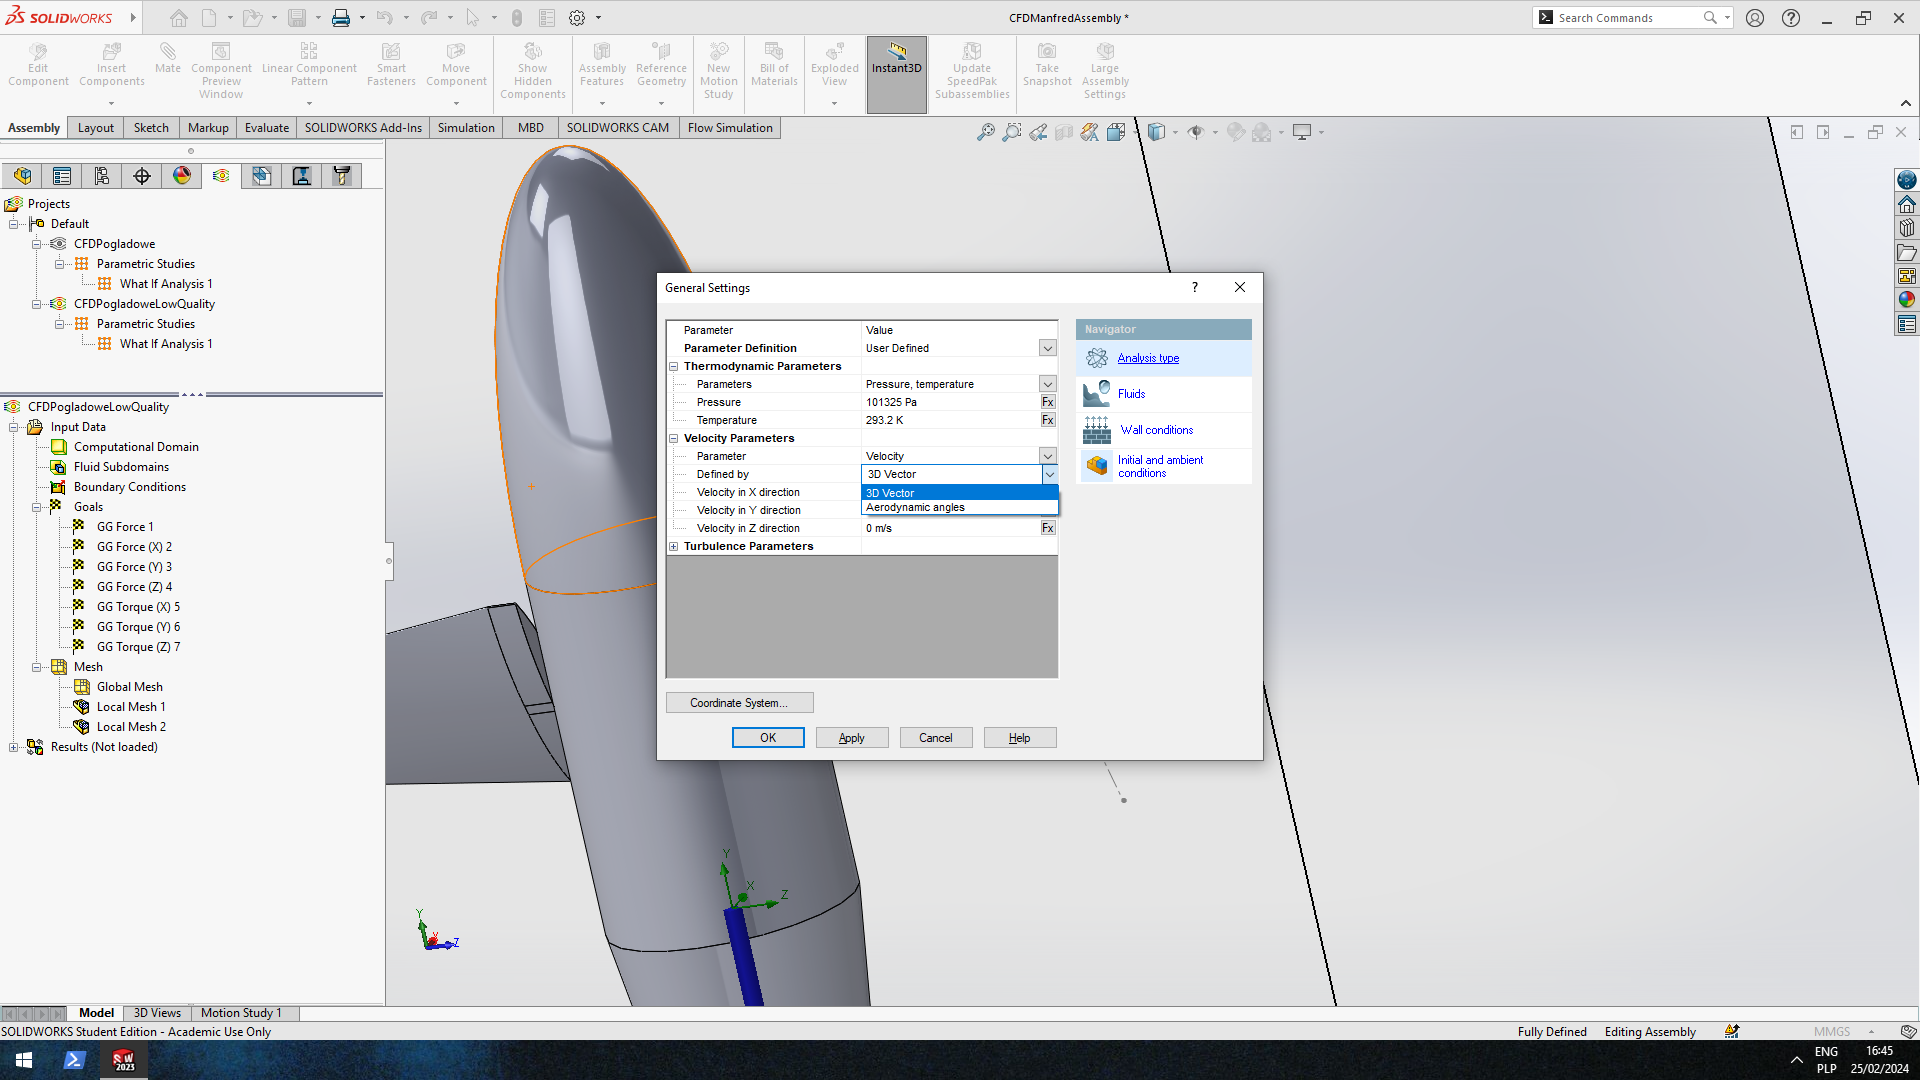
\includegraphics[width=\textwidth]{ATTACK/3Dvector.png}
    \caption{Sternik 1.5 model}
\end{figure}

\begin{figure}[H]
    \centering
    \includegraphics[width=\textwidth]{ATTACK/img1.png}
    \caption{Sternik 1.5 model}
\end{figure}

\begin{figure}[H]
    \centering
    \includegraphics[width=0.8\textwidth]{ATTACK/img2.png}
    \caption{Sternik 1.5 model}
\end{figure}

\begin{figure}[H]
    \centering
    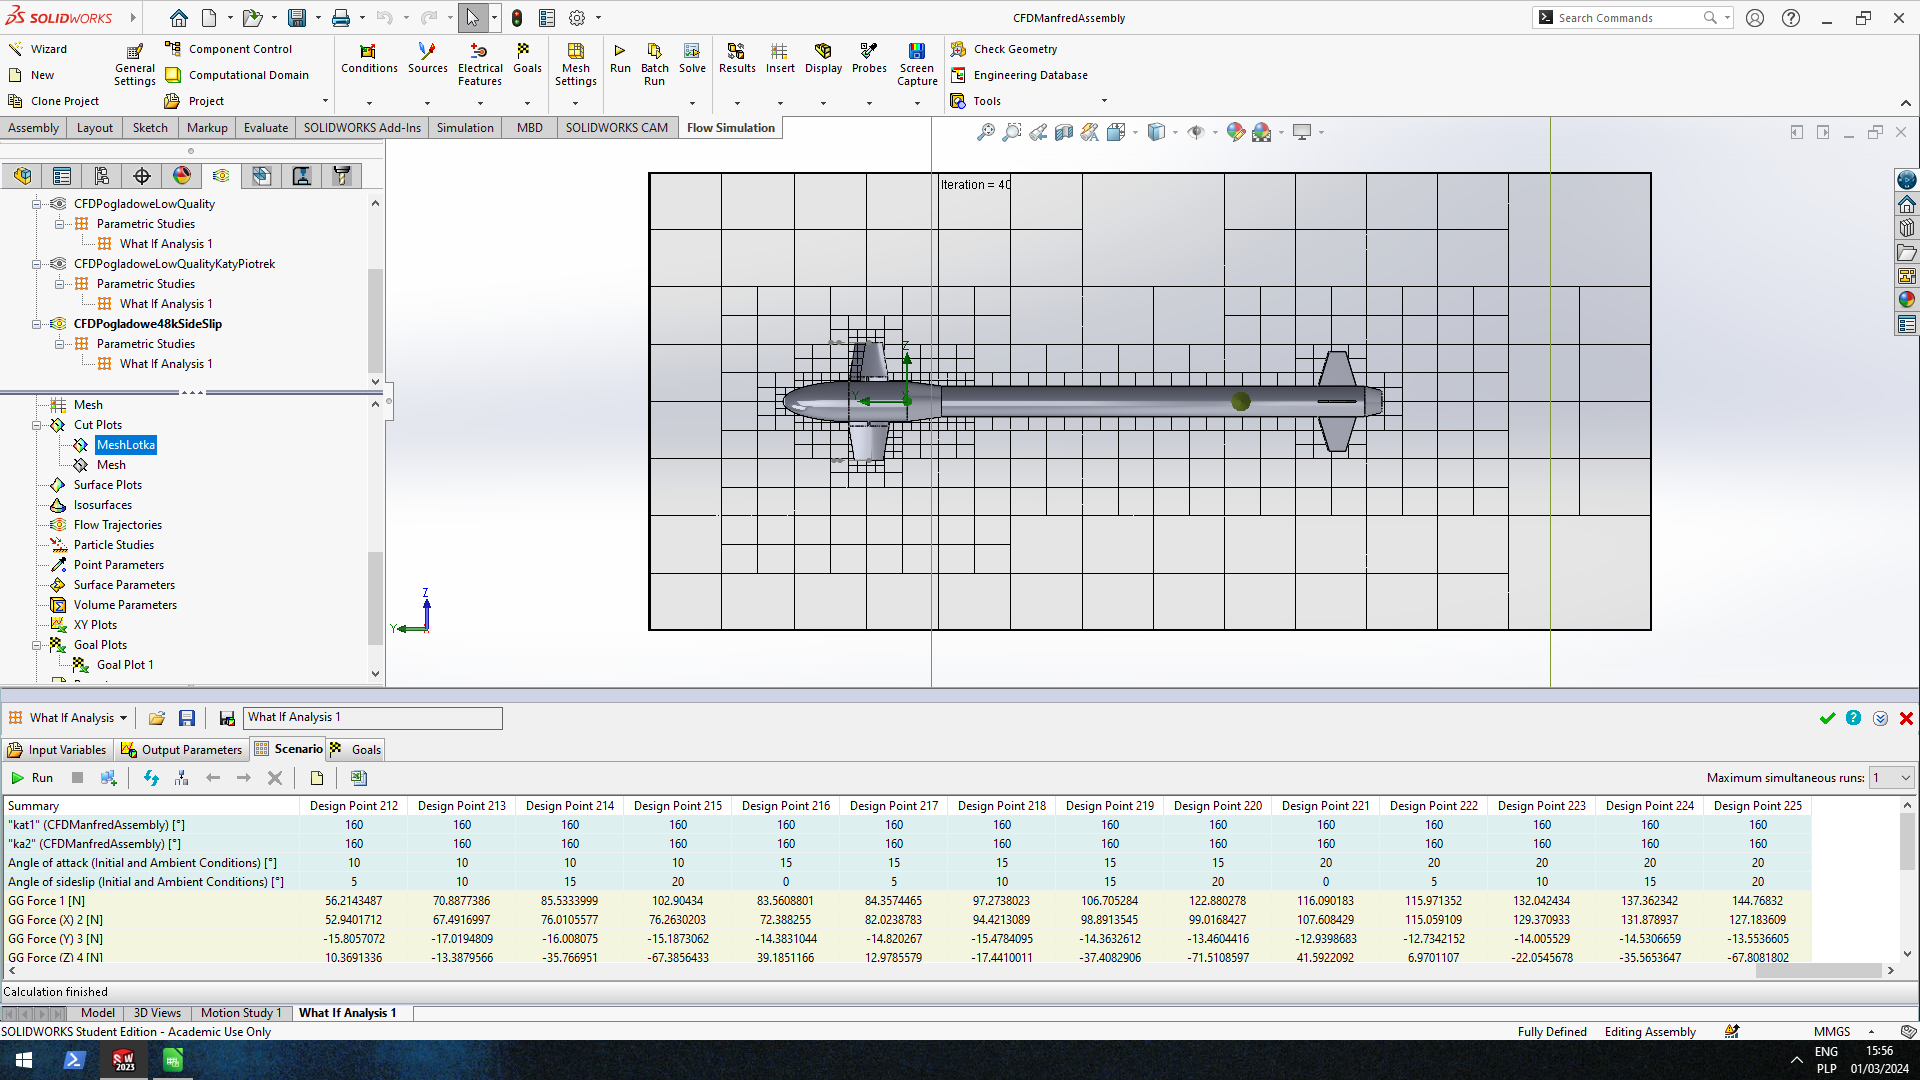
\includegraphics[width=0.8\textwidth]{ATTACK/img3.png}
    \caption{Sternik 1.5 model}
\end{figure}
\newpage
\section{Important problem with Solidworks}
For some reason, when testing and analysing simulations for attack of 10 degrees, problems with 
non-symetrical turbulences started to appear. After analysing the problem, it was found that
changing the point of the beggining of the coordinate system to peak of the model solved the
problem. \\\\
However, later when parametric studies for angles of attack were made, some unexpected results
appeared. Those resoults were significaly different from ones accuired for earlier assembly.\\\\
This was finaly the reason why we stoped for some time working with Solidworks and decided that 
Ansys is a better tool for this kind of simulations. 

\begin{figure}[H]
    \centering
    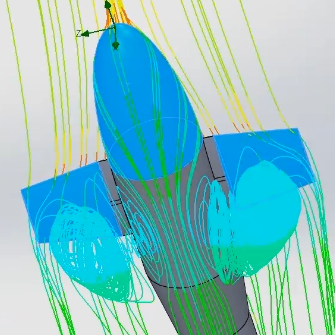
\includegraphics[width=0.5\textwidth]{ATTACK/img4.png}
    \caption{Symetrical turbulences for new assembly}
\end{figure}

\begin{figure}[H]
    \centering
    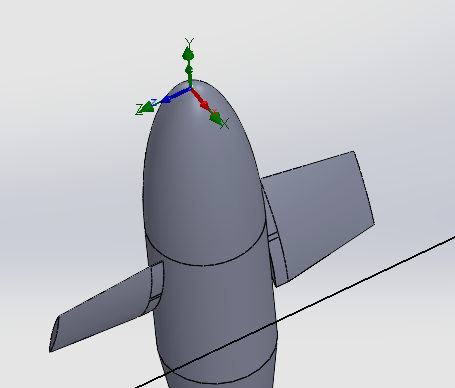
\includegraphics[width=0.5\textwidth]{ATTACK/img5.png}
    \caption{New assembly}
\end{figure}

\section{Parametric study for Sternik 1.5 with angle of attack and sideslip by Piotrek}
Here is where problems started to arise with Solidworks. Simulations for the attack angle As
were made, but the results were not as expected. Bellow are the graphs for the study. \\\\
The results are in the PiotrekSymulacje2702.opju file.

\subsection{Canard angles of (20, 20) degrees}
This results seem to make sense, howerver are still very hard to imagine. This one is for the
mesh of 93k cells. 

\begin{figure}[H]
    \centering
    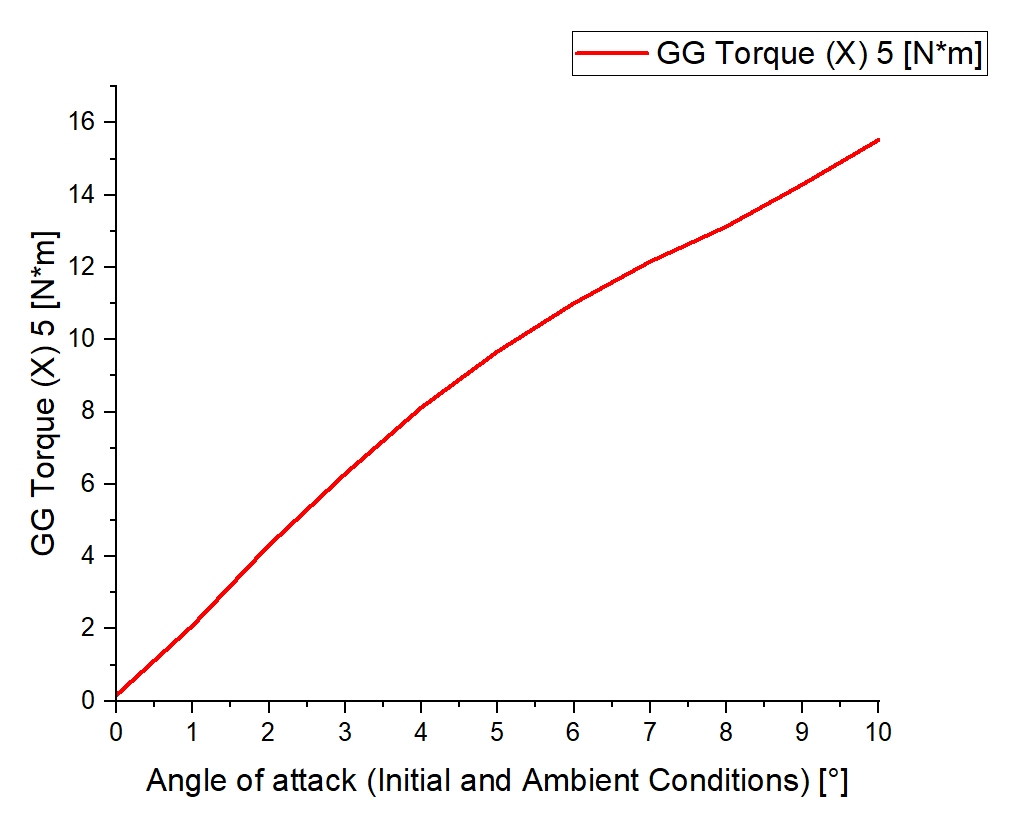
\includegraphics[width=0.8\textwidth]{AttackPiotrek/20x20torqueX.png}
    \caption{Sternik 1.5 model}
\end{figure}

\begin{figure}[H]
    \centering
    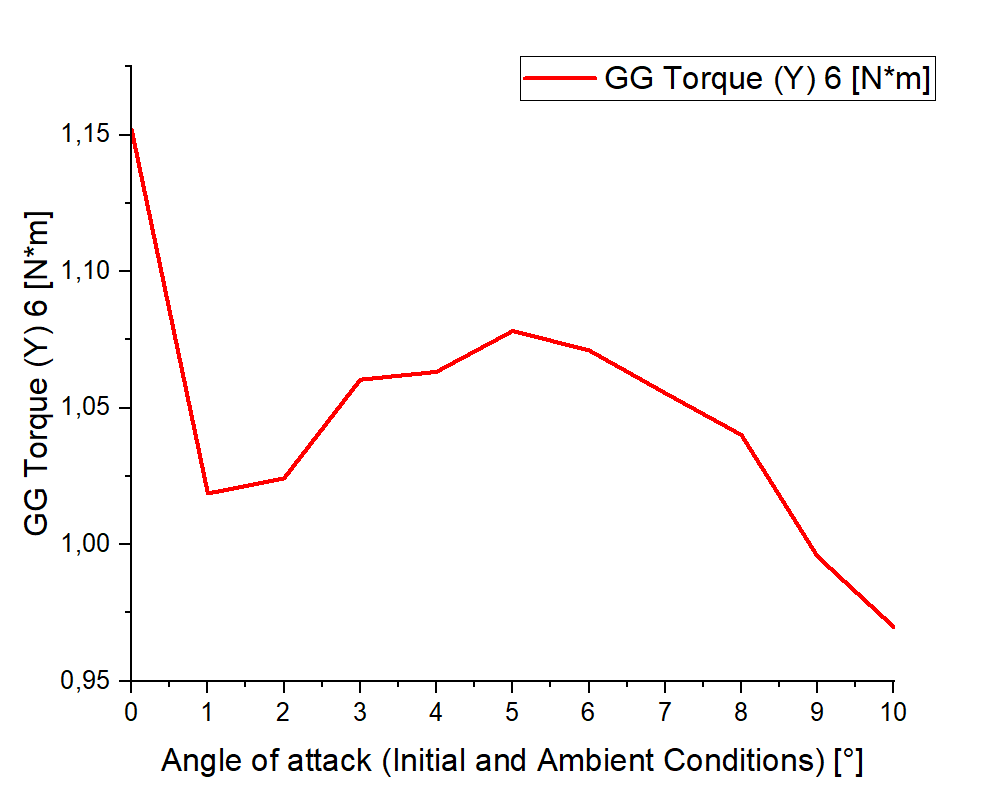
\includegraphics[width=0.75\textwidth]{AttackPiotrek/20x20torqueY.png}
    \caption{Sternik 1.5 model}
\end{figure}

\begin{figure}[H]
    \centering
    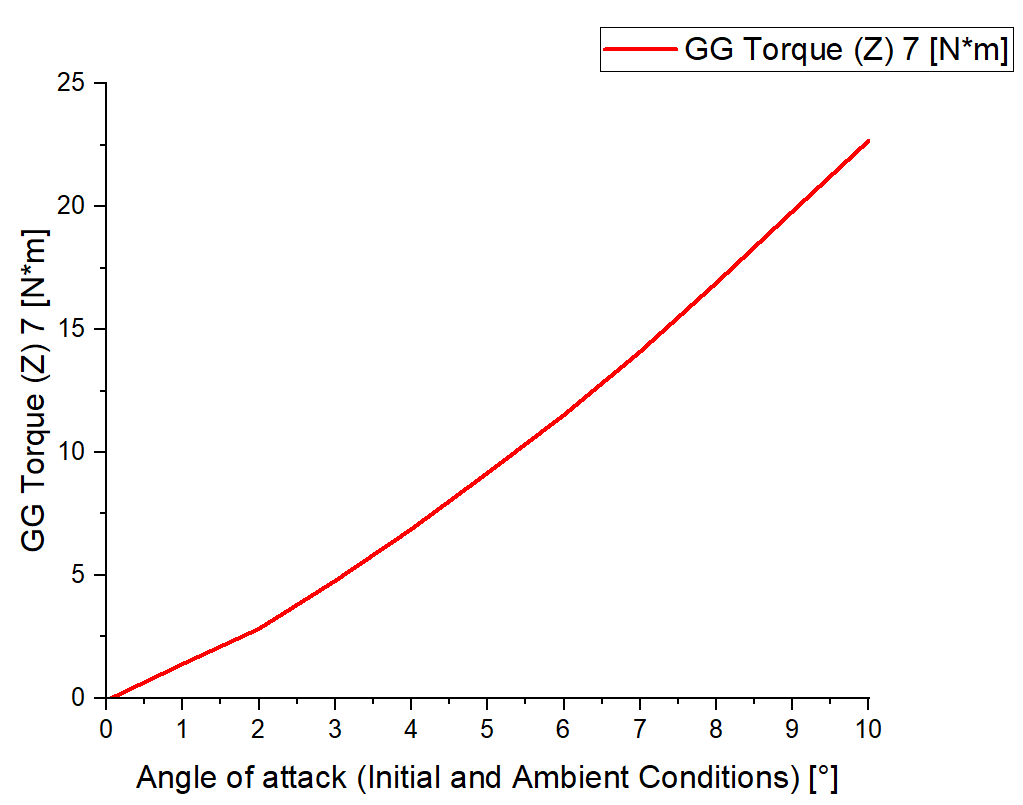
\includegraphics[width=0.75\textwidth]{AttackPiotrek/20x20torqueZ.png}
    \caption{Sternik 1.5 model}
\end{figure}

\subsection{Canard angles of (0, 0) degrees}
This one seems to be the way we predicted, however you can see wild fluctuations in torque X.

\begin{figure}[H]
    \centering
    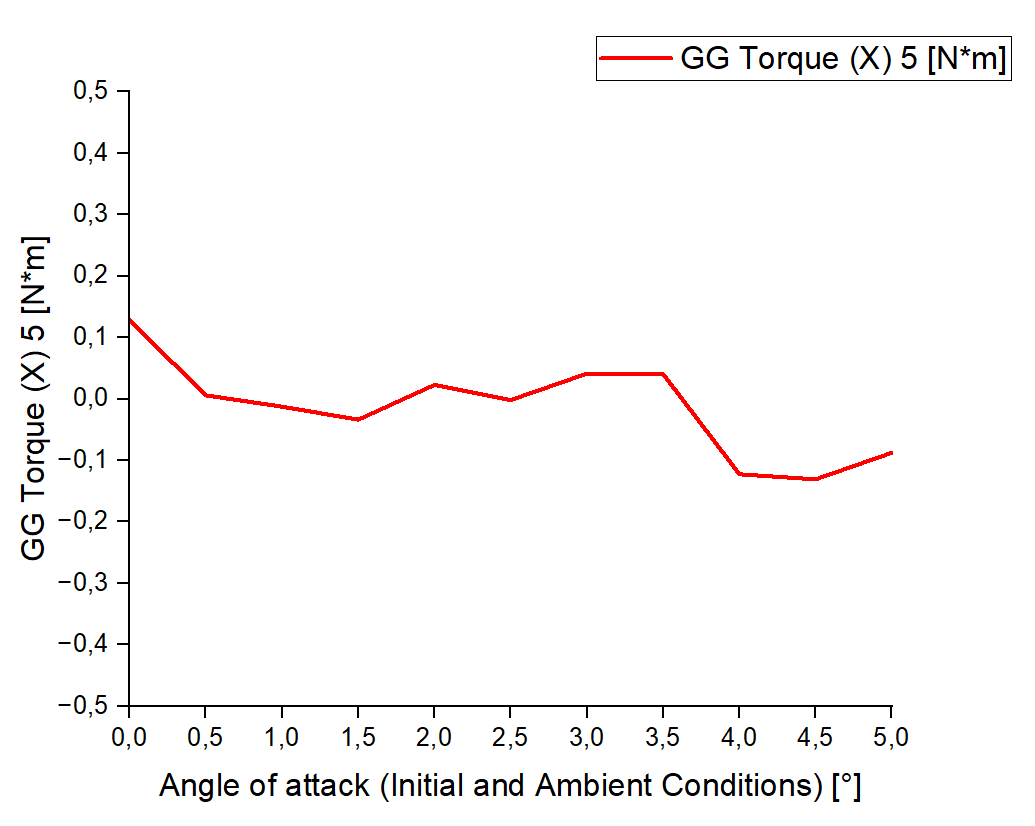
\includegraphics[width=0.7\textwidth]{AttackPiotrek/0x0torqueX.png}
    \caption{Sternik 1.5 model}
\end{figure}

\begin{figure}[H]
    \centering
    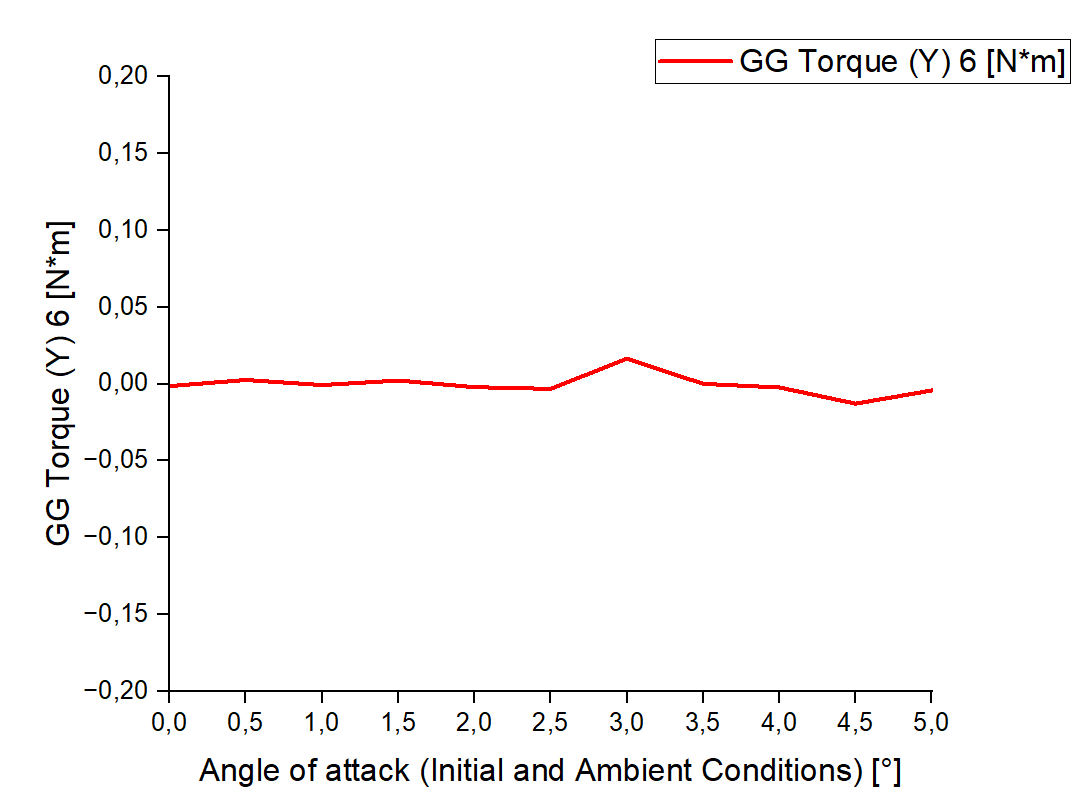
\includegraphics[width=0.7\textwidth]{AttackPiotrek/0x0torqueY.png}
    \caption{Sternik 1.5 model}
\end{figure}

\begin{figure}[H]
    \centering
    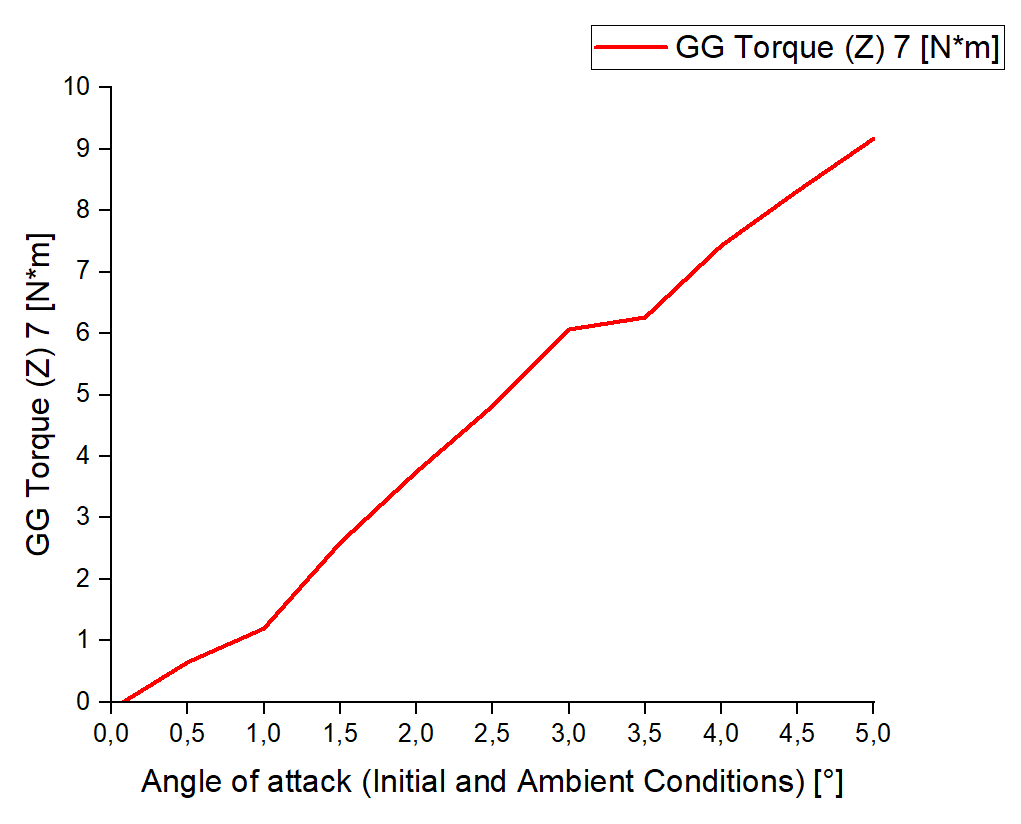
\includegraphics[width=0.8\textwidth]{AttackPiotrek/0x0torqueZ.png}
    \caption{Sternik 1.5 model}
\end{figure}
\newpage
\section{The problematic (0, 20) degrees study}
This time it was JOVER. The results were very strange and we couldnt understand them. 
Those were just wrong. Especially the torque Z, which for angle of attack of 0 degrees 
had value of 0. \\\\
Also the graph for torque X was "heresy" as Piotrek said. \\\\
Later I remade the study with different mesh, but the results were the same. This
meant that either we had no idea about what we got, and what we should have gotten or 
something went wrong.\\\\
Btw the mesh was still 93k cells. \\\\
This one was also redone by me for same assembly, but with different mesh, however resoults were still
flawed.
\newpage
\begin{figure}[H]
    \centering
    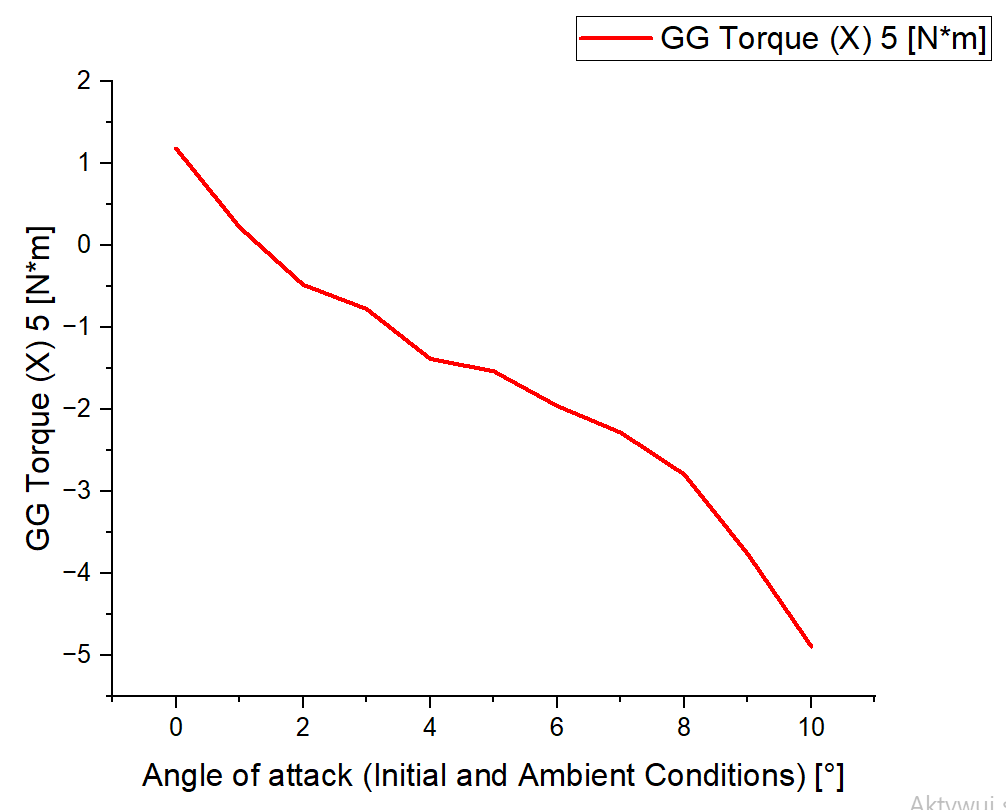
\includegraphics[width=0.7\textwidth]{AttackPiotrek/0x20torqueX.png}
    \caption{Sternik 1.5 model}
\end{figure}

\begin{figure}[H]
    \centering
    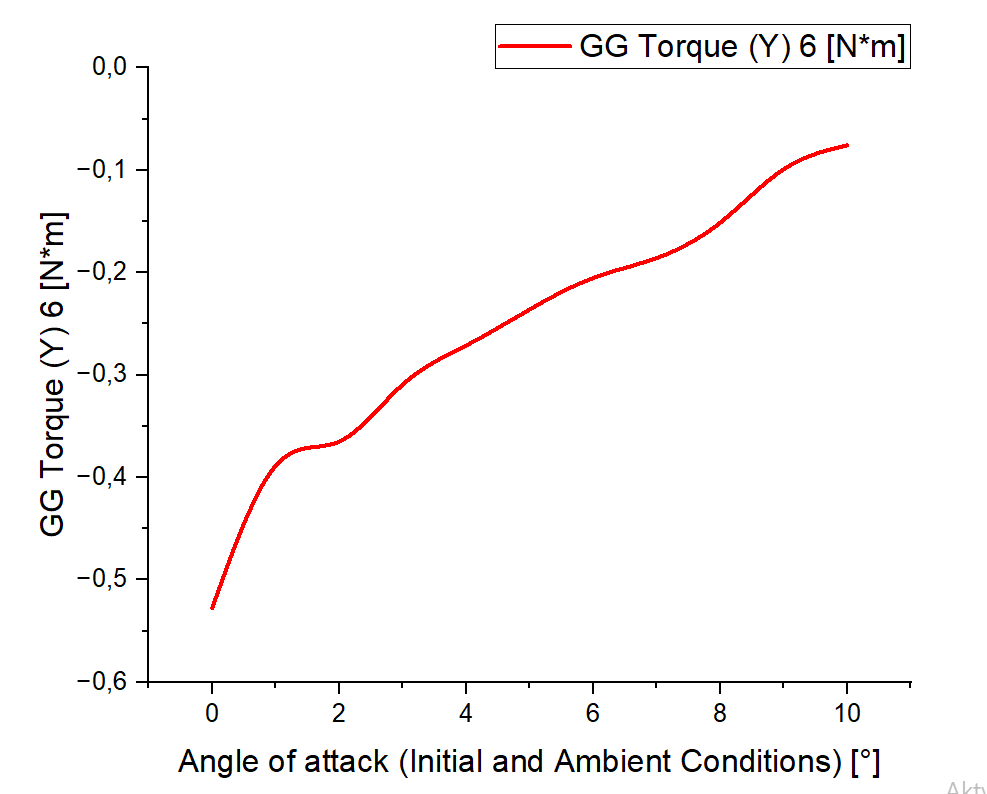
\includegraphics[width=0.7\textwidth]{AttackPiotrek/0x20torqueY.png}
    \caption{Sternik 1.5 model}
\end{figure}

\begin{figure}[H]
    \centering
    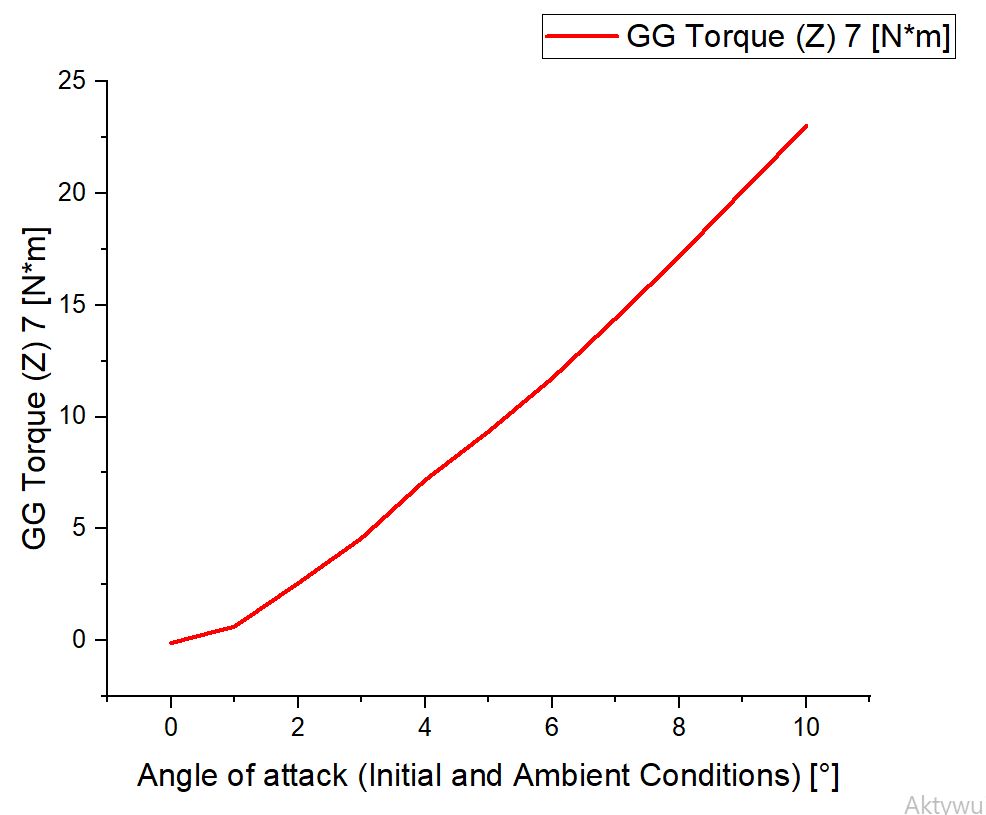
\includegraphics[width=0.8\textwidth]{AttackPiotrek/0x20torqueZ.png}
    \caption{Sternik 1.5 model}
\end{figure}

\begin{figure}[H]
    \centering
    \includegraphics[width=0.8\textwidth]{AttackPiotrek/img1.png}
    \caption{Sternik 1.5 model}
\end{figure}

\begin{figure}[H]
    \centering
    \includegraphics[width=0.7\textwidth]{AttackPiotrek/img2.png}
    \caption{Sternik 1.5 model}
\end{figure}

\section{Same (0, 20) study on the old assembly}
As the results were very strange, I decided to remake the study on the old assembly. 
Values of torques will varry, since the point of the coordinate system was changed, but overall
change in the values should be the same. Also take into note that my study was low quality, so 
fluctuations may be high.\\\\
Quick note, mesh was 12k cells and I used other candard so the look at those with perspective of
them being symetrical to ones before.

\begin{figure}[H]
    \centering
    \includegraphics[width=0.4\textwidth]{AttackManfred/img1.png}
    \caption{Piotrek's angles}
\end{figure}

\begin{figure}[H]
    \centering
    \includegraphics[width=0.8\textwidth]{AttackManfred/img2.png}
    \caption{Manfred's angles}
\end{figure}

\begin{figure}[H]
    \centering
    \includegraphics[width=0.8\textwidth]{AttackManfred/torqueX.png}
    \caption{Sternik 1.5 model}
\end{figure}

\begin{figure}[H]
    \centering
    \includegraphics[width=0.8\textwidth]{AttackManfred/torqueY.png}
    \caption{Sternik 1.5 model}
\end{figure}

\begin{figure}[H]
    \centering
    \includegraphics[width=0.8\textwidth]{AttackManfred/torqueZ.png}
    \caption{Sternik 1.5 model}
\end{figure}

\subsection{Comparison of the results}
As you can see, the results are symetrical for the torque X and Y, but the torque Z is not. 
Also, for this assembly, the torque Z for angle of attack of 0 degrees is not 0 and in general
graph is a lot more probable than for the new assembly. \\\\
This means that the new assembly is not good for parametric studies, but honestly we have no idea
why.

\subsection{Same cannard on new assembly by Piotrek}

\begin{figure}[H]
    \centering
    \includegraphics[width=0.7\textwidth]{AttackManfred/1torqueX.png}
    \caption{WHOPA GAMMA STYLE}
\end{figure}

\begin{figure}[H]
    \centering
    \includegraphics[width=0.7\textwidth]{AttackManfred/1torqueY.png}
    \caption{Sternik 1.5 model}
\end{figure}

\begin{figure}[H]
    \centering
    \includegraphics[width=0.8\textwidth]{AttackManfred/1torqueZ.png}
    \caption{Sternik 1.5 model}
\end{figure}
\newpage
\section{Parametric for angles of cannards for angle of attack of 0 degrees by Piotrek}
For X and Y it makes sense, but for Z it doesnt. Goodnight.

\begin{figure}[H]
    \centering
    \includegraphics[width=0.7\textwidth]{newAssemblyPiotrek/torqueX.png}
    \caption{Sternik 1.5 model}
\end{figure}

\begin{figure}[H]
    \centering
    \includegraphics[width=0.7\textwidth]{newAssemblyPiotrek/torqueY.png}
    \caption{Sternik 1.5 model}
\end{figure}

\begin{figure}[H]
    \centering
    \includegraphics[width=0.8\textwidth]{newAssemblyPiotrek/torqueZ.png}
    \caption{Sternik 1.5 model}
\end{figure}

\begin{figure}[H]
    \centering
    \includegraphics[width=\textwidth]{newAssemblyPiotrek/funi.png}
    \caption{Piotrek is on grindset}
\end{figure}
\newpage
\section{Why not use global angles for parametric studies}
After that I did huge study for  angles of attack and sideslip for (0,0), (0, 20), (20, 20) and 
(20, 0) degrees of cannards. I won't dive into the results, since it's too much and we didn't
even bother to analyze them. \\\\
However here we noticed that if you use global angles for parametric studies, when changing the
angle of attack and the angle of sideslip mesh will change. And it well change in a way that
if you have 24k for (0, 0) degrees, you will have maybe 4k for (0, 20) degrees. \\\\
And I don't have to explaing that for mesh 4k, your results will be very different from reality. 
Underneath you can see cells for the same mesh setting in the same parametric study.\\\\
If for some reason someone CRAZY will want to see the resoults, they are in the 
ParametricStudy48kNatarcie.xlsx file and graphs in opracowanie48kNatarcie.opju file.

\begin{figure}[H]
    \centering
    \includegraphics[width=\textwidth]{meshFuni/img1.png}
    \caption{lalala}
\end{figure}

\begin{figure}[H]
    \centering
    \includegraphics[width=\textwidth]{meshFuni/img2.png}
    \caption{lalala}
\end{figure}

\begin{figure}[H]
    \centering
    \includegraphics[width=\textwidth]{meshFuni/img3.png}
    \caption{lalala}
\end{figure}

\section{Conclusion}
Solidworks is a great tool for simple simulations, but for more complex ones, it's not the best.
Also, the parametric studies here are simple to learn, so its a good tool for beggining. \\\\
However, in the end we decided to focus on pushing forward with Ansys, since it's a better tool for
this kind of simulations and we had 2 major problems with Solidworks:
\begin{itemize}
    \item Problems with symetries in turbulences
    \item Problems with mesh scaling down when changing angles of attack and sideslip
\end{itemize}
However it's simple to fix the secound one, just do the angles of attack and sideslip in the
assemply in same way that you do the cannard angles. 

